\subsection{Jefferson's Method}

\content{
        \begin{definition}
        \begin{itemize}
        \item Find the Standard divisor
        \item Find each states lower quota
        \item If the lower quotas do not add up to the number of seats
        available, then adjust the divisor, and go back to step 2. 
        \end{itemize}
        \end{definition}
}{% presentation
}{% nopresentation
}{% comments
}

\content{
        \begin{example} Let's redo the first example from last time, this time
        with Jefferson's method. \\
        \begin{tabular}{lr}
        County & Population \\
        \hline
        Kent & 162,310 \\
        New Castle & 538,479 \\
        Sussex & 197,145 \\
        \hline
        Total & 1,052,567
        \end{tabular}
        \end{example}
}{% presentation
\vspace{3in}
}{% nopresentation
\vspace{3in}
}{% comments
}

\content{
        \begin{example} Use Jefferson's method to apportion the 75 seats of Rhode
        Island's House of Representatives amoung it's five counties. \\
        \begin{tabular}{lr}
        County & Population \\
        \hline
        Brisol & 49,875 \\
        Kent & 166,158\\
        Newport & 82,888 \\
        Providence & 626,667\\
        Washington & 126,979 \\
        \hline
        Total & 1,052,567
        \end{tabular}
        \end{example}
}{% presentation
\vspace{4in}
}{% nopresentation
\vspace{4in}
}{% comments
}

\content{
        \begin{example}
        Three peaople invest in a treasure dive, each investing the amount
        listed below. The dive results in 36 gold coins. Apportion those coins
        to the investors using Jefferson's method. \\
        \begin{tabular}{lr}
        Alice & \$7,600 \\
        Ben: & \$5,900 \\
        Calos: & \$1,400
        \end{tabular}
        \end{example}
}{% presentation
\vspace{3in}
}{% nopresentation
\vspace{3in}
}{% comments
}


\subsection{Apportionment of Legislative Districts}

\content{
        In most states, rather than apportioning each county a number of
        representatives, districts are drawn so that each legislator represents
        a district. Therefore, the apportionment process happens by drawing the
        districts themselves. Unfortunately, the process of redistricting is
        typically done by the legislature itself, so we often see
        \textbf{gerrymandering}.

        \begin{definition} \textbf{Gerrymandering} is when districts are drawn
        based on the political affiliation of the constituents to the advantage
        of those drawing the boundary. 
        \end{definition}
        
}{% presentation
}{% nopresentation
}{% comments
}

\content{
        \begin{example} Suppose that based on previous voting patters, you
        predict that the city in which you live (which is a perfect rectangle!)
        will vote according to the picture below:  

        \begin{minipage}[t]{0.65\textwidth}
        \vspace{0pt}
        There is an election coming up, and you are a legislator in the yellow
        party. Luckily, you are in charge of redistricting the city into 5
        districts before the next upcoming election. Can you find 5 districts
        so that
        \begin{itemize}
        \item Each district must contain at least one yellow square and at least
        one blue square, and 
        \item 3 of the 5 districts will vote yellow (there are more yellow
        squares than blue ones in that district)?
        \end{itemize}
        \end{minipage}\hfill\begin{minipage}[t]{0.25\textwidth}
        \vspace{0pt}
        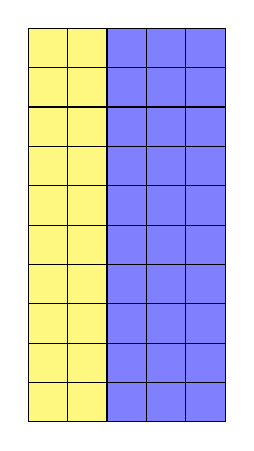
\begin{tikzpicture}[scale=0.5]
        \foreach \x in {0,1} {
                \foreach \y in {0,1,2,3,4,5,6,7,8,9} {
                        \draw[fill=yellow!50] (\x,\y) rectangle (\x+1,\y+1);
                }
        }
        \foreach \x in {2,3,4} {
                \foreach \y in {0,1,2,3,4,5,6,7,8,9} {
                        \draw[fill=blue!50] (\x,\y) rectangle (\x+1,\y+1);
                }
        }
        \end{tikzpicture}
        \end{minipage}
        \end{example}
}{% presentation
}{% nopresentation
}{% comments
}
